% Options for packages loaded elsewhere
\PassOptionsToPackage{unicode}{hyperref}
\PassOptionsToPackage{hyphens}{url}
%
\documentclass[
  man]{apa7}
\usepackage{amsmath,amssymb}
\usepackage{lmodern}
\usepackage{iftex}
\ifPDFTeX
  \usepackage[T1]{fontenc}
  \usepackage[utf8]{inputenc}
  \usepackage{textcomp} % provide euro and other symbols
\else % if luatex or xetex
  \usepackage{unicode-math}
  \defaultfontfeatures{Scale=MatchLowercase}
  \defaultfontfeatures[\rmfamily]{Ligatures=TeX,Scale=1}
\fi
% Use upquote if available, for straight quotes in verbatim environments
\IfFileExists{upquote.sty}{\usepackage{upquote}}{}
\IfFileExists{microtype.sty}{% use microtype if available
  \usepackage[]{microtype}
  \UseMicrotypeSet[protrusion]{basicmath} % disable protrusion for tt fonts
}{}
\makeatletter
\@ifundefined{KOMAClassName}{% if non-KOMA class
  \IfFileExists{parskip.sty}{%
    \usepackage{parskip}
  }{% else
    \setlength{\parindent}{0pt}
    \setlength{\parskip}{6pt plus 2pt minus 1pt}}
}{% if KOMA class
  \KOMAoptions{parskip=half}}
\makeatother
\usepackage{xcolor}
\usepackage{graphicx}
\makeatletter
\def\maxwidth{\ifdim\Gin@nat@width>\linewidth\linewidth\else\Gin@nat@width\fi}
\def\maxheight{\ifdim\Gin@nat@height>\textheight\textheight\else\Gin@nat@height\fi}
\makeatother
% Scale images if necessary, so that they will not overflow the page
% margins by default, and it is still possible to overwrite the defaults
% using explicit options in \includegraphics[width, height, ...]{}
\setkeys{Gin}{width=\maxwidth,height=\maxheight,keepaspectratio}
% Set default figure placement to htbp
\makeatletter
\def\fps@figure{htbp}
\makeatother
\setlength{\emergencystretch}{3em} % prevent overfull lines
\providecommand{\tightlist}{%
  \setlength{\itemsep}{0pt}\setlength{\parskip}{0pt}}
\setcounter{secnumdepth}{-\maxdimen} % remove section numbering
% Make \paragraph and \subparagraph free-standing
\ifx\paragraph\undefined\else
  \let\oldparagraph\paragraph
  \renewcommand{\paragraph}[1]{\oldparagraph{#1}\mbox{}}
\fi
\ifx\subparagraph\undefined\else
  \let\oldsubparagraph\subparagraph
  \renewcommand{\subparagraph}[1]{\oldsubparagraph{#1}\mbox{}}
\fi
\newlength{\cslhangindent}
\setlength{\cslhangindent}{1.5em}
\newlength{\csllabelwidth}
\setlength{\csllabelwidth}{3em}
\newlength{\cslentryspacingunit} % times entry-spacing
\setlength{\cslentryspacingunit}{\parskip}
\newenvironment{CSLReferences}[2] % #1 hanging-ident, #2 entry spacing
 {% don't indent paragraphs
  \setlength{\parindent}{0pt}
  % turn on hanging indent if param 1 is 1
  \ifodd #1
  \let\oldpar\par
  \def\par{\hangindent=\cslhangindent\oldpar}
  \fi
  % set entry spacing
  \setlength{\parskip}{#2\cslentryspacingunit}
 }%
 {}
\usepackage{calc}
\newcommand{\CSLBlock}[1]{#1\hfill\break}
\newcommand{\CSLLeftMargin}[1]{\parbox[t]{\csllabelwidth}{#1}}
\newcommand{\CSLRightInline}[1]{\parbox[t]{\linewidth - \csllabelwidth}{#1}\break}
\newcommand{\CSLIndent}[1]{\hspace{\cslhangindent}#1}
\ifLuaTeX
\usepackage[bidi=basic]{babel}
\else
\usepackage[bidi=default]{babel}
\fi
\babelprovide[main,import]{english}
% get rid of language-specific shorthands (see #6817):
\let\LanguageShortHands\languageshorthands
\def\languageshorthands#1{}
% Manuscript styling
\usepackage{upgreek}
\captionsetup{font=singlespacing,justification=justified}

% Table formatting
\usepackage{longtable}
\usepackage{lscape}
% \usepackage[counterclockwise]{rotating}   % Landscape page setup for large tables
\usepackage{multirow}		% Table styling
\usepackage{tabularx}		% Control Column width
\usepackage[flushleft]{threeparttable}	% Allows for three part tables with a specified notes section
\usepackage{threeparttablex}            % Lets threeparttable work with longtable

% Create new environments so endfloat can handle them
% \newenvironment{ltable}
%   {\begin{landscape}\centering\begin{threeparttable}}
%   {\end{threeparttable}\end{landscape}}
\newenvironment{lltable}{\begin{landscape}\centering\begin{ThreePartTable}}{\end{ThreePartTable}\end{landscape}}

% Enables adjusting longtable caption width to table width
% Solution found at http://golatex.de/longtable-mit-caption-so-breit-wie-die-tabelle-t15767.html
\makeatletter
\newcommand\LastLTentrywidth{1em}
\newlength\longtablewidth
\setlength{\longtablewidth}{1in}
\newcommand{\getlongtablewidth}{\begingroup \ifcsname LT@\roman{LT@tables}\endcsname \global\longtablewidth=0pt \renewcommand{\LT@entry}[2]{\global\advance\longtablewidth by ##2\relax\gdef\LastLTentrywidth{##2}}\@nameuse{LT@\roman{LT@tables}} \fi \endgroup}

% \setlength{\parindent}{0.5in}
% \setlength{\parskip}{0pt plus 0pt minus 0pt}

% Overwrite redefinition of paragraph and subparagraph by the default LaTeX template
% See https://github.com/crsh/papaja/issues/292
\makeatletter
\renewcommand{\paragraph}{\@startsection{paragraph}{4}{\parindent}%
  {0\baselineskip \@plus 0.2ex \@minus 0.2ex}%
  {-1em}%
  {\normalfont\normalsize\bfseries\itshape\typesectitle}}

\renewcommand{\subparagraph}[1]{\@startsection{subparagraph}{5}{1em}%
  {0\baselineskip \@plus 0.2ex \@minus 0.2ex}%
  {-\z@\relax}%
  {\normalfont\normalsize\itshape\hspace{\parindent}{#1}\textit{\addperi}}{\relax}}
\makeatother

% \usepackage{etoolbox}
\makeatletter
\patchcmd{\HyOrg@maketitle}
  {\section{\normalfont\normalsize\abstractname}}
  {\section*{\normalfont\normalsize\abstractname}}
  {}{\typeout{Failed to patch abstract.}}
\patchcmd{\HyOrg@maketitle}
  {\section{\protect\normalfont{\@title}}}
  {\section*{\protect\normalfont{\@title}}}
  {}{\typeout{Failed to patch title.}}
\makeatother

\usepackage{xpatch}
\makeatletter
\xapptocmd\appendix
  {\xapptocmd\section
    {\addcontentsline{toc}{section}{\appendixname\ifoneappendix\else~\theappendix\fi\\: #1}}
    {}{\InnerPatchFailed}%
  }
{}{\PatchFailed}
\keywords{keywords\newline\indent Word count: 2869}
\DeclareDelayedFloatFlavor{ThreePartTable}{table}
\DeclareDelayedFloatFlavor{lltable}{table}
\DeclareDelayedFloatFlavor*{longtable}{table}
\makeatletter
\renewcommand{\efloat@iwrite}[1]{\immediate\expandafter\protected@write\csname efloat@post#1\endcsname{}}
\makeatother
\usepackage{csquotes}
\makeatletter
\renewcommand{\paragraph}{\@startsection{paragraph}{4}{\parindent}%
  {0\baselineskip \@plus 0.2ex \@minus 0.2ex}%
  {-1em}%
  {\normalfont\normalsize\bfseries\typesectitle}}

\renewcommand{\subparagraph}[1]{\@startsection{subparagraph}{5}{1em}%
  {0\baselineskip \@plus 0.2ex \@minus 0.2ex}%
  {-\z@\relax}%
  {\normalfont\normalsize\bfseries\itshape\hspace{\parindent}{#1}\textit{\addperi}}{\relax}}
\makeatother

\ifLuaTeX
  \usepackage{selnolig}  % disable illegal ligatures
\fi
\IfFileExists{bookmark.sty}{\usepackage{bookmark}}{\usepackage{hyperref}}
\IfFileExists{xurl.sty}{\usepackage{xurl}}{} % add URL line breaks if available
\urlstyle{same} % disable monospaced font for URLs
\hypersetup{
  pdftitle={The effect of response options on gender categorization ( provisional title)},
  pdfauthor={Elli van Berlekom1 \& Coauthors1,2},
  pdflang={en-EN},
  pdfkeywords={keywords},
  hidelinks,
  pdfcreator={LaTeX via pandoc}}

\title{The effect of response options on gender categorization ( provisional title)}
\author{Elli van Berlekom\textsuperscript{1} \& Coauthors\textsuperscript{1,2}}
\date{}


\shorttitle{Rsponse options and gender categorization}

\authornote{

Add complete departmental affiliations for each author here. Each new line herein must be indented, like this line.

Data \& scripts are available at osf link. The authors declare no conflict of interest.

The authors made the following contributions. Elli van Berlekom: Conceptualization, Writing - Original Draft Preparation, Writing - Review \& Editing; Coauthors: A lot of things, Author order TBD.

Correspondence concerning this article should be addressed to Elli van Berlekom, Albanovägen 12. E-mail: \href{mailto:elli.vanberlekom@psychology.su.se}{\nolinkurl{elli.vanberlekom@psychology.su.se}}

}

\affiliation{\vspace{0.5cm}\textsuperscript{1} Stockholm University\\\textsuperscript{2} Lund University}

\abstract{%
I'm using a premade template \& leaving some of their guidlines in place to help me.

One or two sentences providing a \textbf{basic introduction} to the field, comprehensible to a scientist in any discipline.

Two to three sentences of \textbf{more detailed background}, comprehensible to scientists in related disciplines.

One sentence clearly stating the \textbf{general problem} being addressed by this particular study.

One sentence summarizing the main result (with the words ``\textbf{here we show}'' or their equivalent).

Two or three sentences explaining what the \textbf{main result} reveals in direct comparison to what was thought to be the case previously, or how the main result adds to previous knowledge.

One or two sentences to put the results into a more \textbf{general context}.

Two or three sentences to provide a \textbf{broader perspective}, readily comprehensible to a scientist in any discipline.
}



\begin{document}
\maketitle

Precision is key when measuring constructs in psychological research. One domain where precision is lacking is in the use of binary response options for gender, which fails to capture the complex and fluid nature of gender/sex. The gender binary is most clear in terms of legal gender, where the alternatives in most countries are confined to women or men, this dichotomy does not accurately reflect the diverse biological and self-perceived gender identities that exist (Lindqvist et al., 2019; Hyde et al., 2019). While more flexible options for self-definition of gender identity has become more common in research, the use of non-binary gender options in stimuli and participant response measures remains limited. In light of this, the current study aims to highlight non-binary alternatives to measuring gender categorization and investigate how gender perception is influenced by such non-binary options.

Alternative approaches to binary self-classification of gender have a deep history in psychology. For example, Bem (1974) developed scales to measure femininity and masculinity as separate traits, finding that many individuals exhibit a mixture of feminine and masculine traits. More recently, Joel and colleagues (2014) not only asked participants which gender category they identified with, but also whether they had ever experienced a different gender identity. They found that approximately 30\% of respondents had experienced an alternative gender identity at some point in their lives. Additionally, several guides have been developed that recommend the use of open textboxes or multiple options when asking participants to indicate their gender. When participants are given such textboxes, they frequently used them. Thes studies suggest not only that alternatives are possible, but also that participants will use them when they have the chance, and potentially, the possibilities around gender change.

In contrast, the literature on gender categorization often treats gender as a binary category. Gender categorization is a cognitive process that occurs when individuals perceive others (ref). Researchers in this field have explored the speed and automaticity of gender perception in faces, as well as which facial features are associated with specific gender categories, such as women and men (ref). Generally, the findings indicate that gender is rapidly and automatically categorized, with facial features such as skin smoothness, jawline, and hair length used to determine gender identity. Lastly, studies in this field have indicated that people percieve faces categorically (Campanella et al., 2001). In other words, However, these studies typically do not address the complex nature of gender or consider alternative response options (ref).

Instead, gender categorization is most often measured through a forced-choice task in which participants are forced to indicate either ``female'' or ``male'' when presented with a face (see, for example, Cloutier et al., 2005; Campanella et al., 2001; Webster et al., 2004; Zhao \& Bentin, 2008). A slightly different approach asks participants to rate faces on a gender scale as a quality, often using ``feminine'' and ``masculine'' as endpoints on a single scale (e.g., D'Ascenzo et al., 2015; others). Despite some variations, therefore literature overwhelmingly presents gender as a binary in studies of gender categorization.

The use of binary gender measures presents significant problems in accurately reflecting the complexity of gender. Such measures reinforce the notion of gender as a binary concept, thereby invalidating non-binary genders. This not only misrepresents the reality of gender but also perpetuates discriminatory attitudes towards non-binary individuals. Consequently, it is imperative to consider alternative measures that acknowledge and respect the diversity of gender identities.

\hypertarget{overview-of-the-present-research}{%
\subsection{Overview of the present research}\label{overview-of-the-present-research}}

Based on the problems with binary measurement, we conducted two experiments to demonstrate alternatives to binary measurement of gender categorization and to investigate how such alternative impact participants results. The purpose of bothg experiment was to answer the following three research quetions.

\emph{Research question 1}: Do people use beyond-binary options when they have them?

\emph{researchg question 2}: Two what extent do beyond-binary responses affect the distribution of woman/man responses?

\emph{Research question 3}: Can response options which do not present the categories of woman and man as oppositional reduce categorical perception.

\hypertarget{experiment-1}{%
\section{Experiment 1}\label{experiment-1}}

The purpose of study 1 was to test research questions 1 and 2. Consequently, experiment 1 focused on manipulating various ways to let particpants catgorize faces beyond the binary of women and me. The specific alternatives were based on common practices for self-identification of gender. To avoid suggesting that gender only consist of women and men, these studies recommend includding a third option. Because gender is not always apparent from someone's face, such a task should also include an ``I don't know option''. The inclusion of such options is sometimes discouraged because it makes participants not taking a stance, however, when it comes to gender, not taking a stance is a legitimate strategy.

A paragraph about free text maybe.

\hypertarget{method}{%
\subsection{Method}\label{method}}

\hypertarget{participants}{%
\subsubsection{Participants}\label{participants}}

Participants (\emph{N} = 68) were recruited through advertising online and on the university campus (\emph{M}\textsubscript{age}= 37.67, \emph{SD}\textsubscript{age} = 14.56, Range = 20 - 69). All participants were informed that participation was voluntary. In term of gender, the participants were 35 women, 32 men and 1 who did not indicate gender. All participants provided written informed consent and were informed that participation was voluntary.

\hypertarget{stimuli}{%
\subsubsection{Stimuli}\label{stimuli}}

Faces were produced using faces from the London Face Database (deBruine) and the Chicago Face Database (ref) morphed with on Webmorph (ref). For Black, Asian and White faces, the six most feminine faces of women and the six most masculine faces of men were selected, using the codebook provided by the researchers. The faces were matched, so that the most feminine face were morphed with the most masculine face and so on. The morphs were made in 7 steps, from completely feminine to completely masculine. Because there were 18 pairs morphed in 7 steps, the total number of faces was 126.

\hypertarget{measures}{%
\subsection{Measures}\label{measures}}

The primary outcome was responses to the categorizatio task. For analysis purposes, these were aggregated in the following ways:

\emph{Beyond-binary responses} represented the categories where participants made a response that were not woman or man. This was a dichotomous variable that was calculated from the categorization data by combining the responses of ``I don't know'' and ``non-binary''. These beyond-binary responses were coded as 1 and binary responses as 0.

\emph{Binary response} represented only the responses that were either woman (coded as 1) or man (coded as 0). All other responses were removed from this dataset.

\hypertarget{procedure}{%
\subsubsection{Procedure}\label{procedure}}

Participants completed the experiment on a computer in a quiet room. Each trial consisted of a face accompanied by the question ``How would you gender categorize this person?''. Each person completed a total of 126 trials. Participants were randomly allocated into one of the three response options conditions: binary categories, multiple categories and free text. In the binary categories condition, the only option to respond was ``woman'' and ``man''. In the multiple categories condition, this was expanded to include the options ``other'' and ``I don't know''. Lastly, the free text condition consisted of an open text box.

\hypertarget{data-analysis}{%
\subsubsection{Data analysis}\label{data-analysis}}

We used R (Version 4.2.2; R Core Team, 2022) and the R-packages \emph{bayesplot} (Version 1.10.0; Gabry et al., 2019), \emph{brms} (Version 2.18.0; Bürkner, 2017, 2018, 2021), \emph{dplyr} (Version 1.0.10; Wickham et al., 2022), \emph{gcookbook} (Version 2.0; Chang, 2018), \emph{ggplot2} (Version 3.4.0; Wickham, 2016), \emph{papaja} (Version 0.1.1; Aust \& Barth, 2022), \emph{Rcpp} (Eddelbuettel \& Balamuta, 2018; Version 1.0.9; Eddelbuettel \& François, 2011), \emph{tidybayes} (Version 3.0.2; Kay, 2022), \emph{tidyr} (Version 1.2.1; Wickham \& Girlich, 2022), and \emph{tinylabels} (Version 0.2.3; Barth, 2022). Descriptive statistics were used to summarize the data, and Bayesian mixed-effects models were used to test the research questions. For all models, we included varying intercepts for both participants and trials. To answer each research question, we used a two-step approach which began with a model comparison approach followed by Bayes factor tests of specific contrasts. In all cases, the models included varying intercepts for both participants trials.

\hypertarget{research-question-1-the-use-of-categories-beyond-the-binary}{%
\paragraph{Research question 1: The use of categories beyond the binary}\label{research-question-1-the-use-of-categories-beyond-the-binary}}

In research question one, we investigated whether participants categorized faces beyond the binary when given the chance. This could manifest as either a main effect of condition or an interaction between condition and morph level if categorizations beyond the binary were limited to only the most androgynous faces. For this analyses, the Binary categories condition was excluded, as that condition preculded the possibility of categorizing beyond the binary. The specific questions then, were ``do people categorize faces beyond the binary?'', ``does this effect depend on condition?'' and ``are ambiguous faces more likely to be categorized beyond the binary?''. These questions correspond to main effects of response option condition, facial morph level and an interaction between the two.

Accordingly, the modelling strategy involved a null model with no additional predictors, a Main effects model and an Interaction model For full model specification (including priors) and diagnostics, see the supplementary material. These model were then compared in terms of predictive power on out-of-sample data points, estimated using Leave-one-out cross validation (LOO-CV). This represents an indirect test of the research questions, and can be viewed as an imperfect analogy to checking whether there is a ``significant'' interaction in a classical F-test.

As a more direct test, we also calculated the Bayes Factor for the specific contrasts suggested by these questions. In other words, we compared the overall probability of making categorizations beyond the binary in the Free text condition and the Multiple categories conditions. Additionally,
we compared the prevalence of categorization beyond the binar specifically of the most androgynous faces. The Bayes factors were compared the null hypothesis that the contrast was equal to 0 and calculated using the Savage-Dickey Density Ratio.

\hypertarget{research-question-2-the-distribution-of-binary-responses}{%
\paragraph{Research question 2: The distribution of binary responses}\label{research-question-2-the-distribution-of-binary-responses}}

In research question two, we investigated whether the distribution of binary responses was different depending on response option condition. This could manifest as a main effect of condition if there was an overall skew in the results or as an interaction between condition and morph level, in case that the skew was isolated to just one level of morph (for example at the middle).

Similar to RQ1, this data was tested using with Bayesian mixed models fitted to the data. This included an initial model comparison approach, with Null model, and Main Effects model and an Interaction Model. If the model comparsion did not preculde the Intearction model, we tested the contrast of the overall distribution as well as isolated to whichever morph level, a visual inspection of the data suggeted was the most strongly skewed.

\hypertarget{results}{%
\section{Results}\label{results}}

\hypertarget{research-question-1-the-use-of-categories-beyond-the-binary-1}{%
\subsection{Research question 1: The use of categories beyond the binary}\label{research-question-1-the-use-of-categories-beyond-the-binary-1}}

The raw distribution of categorizations is presented in Figure~\ref{fig:descriptives}.

\emph{to do: fix the bug that is producing those ugly red lines at the bottom of this figure}

\begin{figure}
\centering
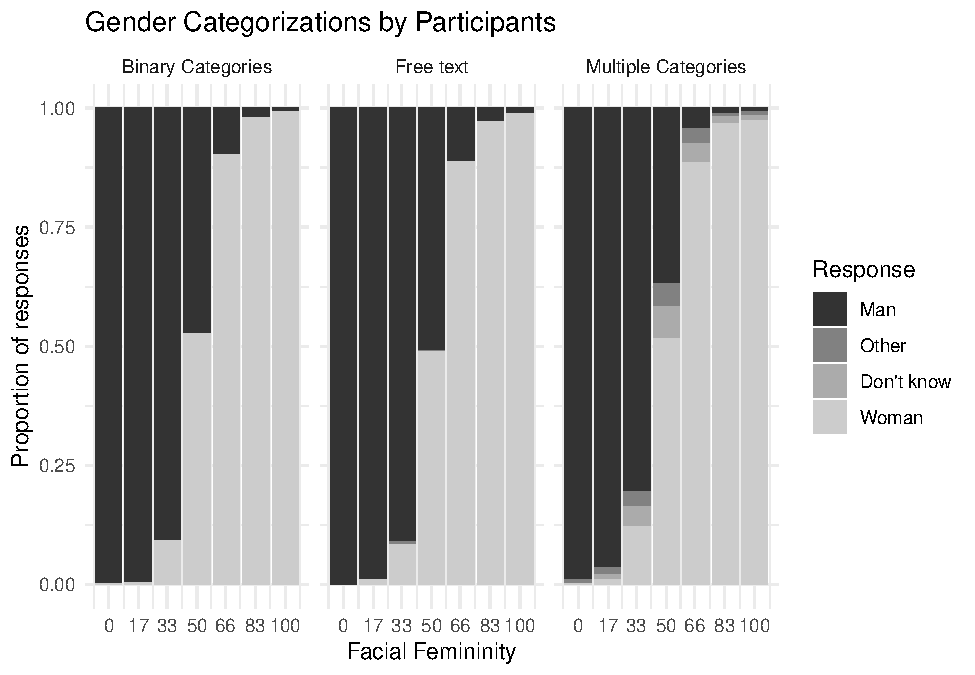
\includegraphics{resp_opts_manus23022_files/figure-latex/descriptives-1.pdf}
\caption{\label{fig:descriptives}Gender Categorizations by Participants}
\end{figure}

As described in the methods, to investigating RQ1 we fit a Null Model, a Main Effects Model and an interaction model to the data. The results of model comparison are presented in Table~\ref{tab:loo}.
Table~\ref{tab:loo} suggests that the Interaction model is the most predictive, but the absolute differnce between the Interaction model and the Main effects model is small and more importantly, the difference is small in relation to the standard error of the difference. This suggests that the data is inconclusive about which model is most suitable, but both are superior to the Null model. As model comparison did not conclusively preclude the Interaction model, we continued by testing specific, relevant contrasts using the Interaction model (see the Supplementary material for specific contrast weights).

\begin{table}

\caption{\label{tab:loo}Relative predictive power of models describing the outcome on the categorization task}
\centering
\begin{threeparttable}
\begin{tabular}[t]{lcccc}
\toprule
  & LOO diff & St. Error diff & LOO & St. Error LOO\\
\midrule
Interaction & 0.00 & 0.00 & -234.17 & 23.23\\
Main Effect & -2.46 & 2.71 & -236.63 & 23.07\\
Null & -18.83 & 6.02 & -253.00 & 24.51\\
\bottomrule
\end{tabular}
\begin{tablenotes}[para]
\item \textit{Note.} 
\item LOO diff refers to the difference in loo between the model and the most predictive model. The first row describes the most predictive model, which is why the difference is 0
\end{tablenotes}
\end{threeparttable}
\end{table}

\begin{figure}
\centering
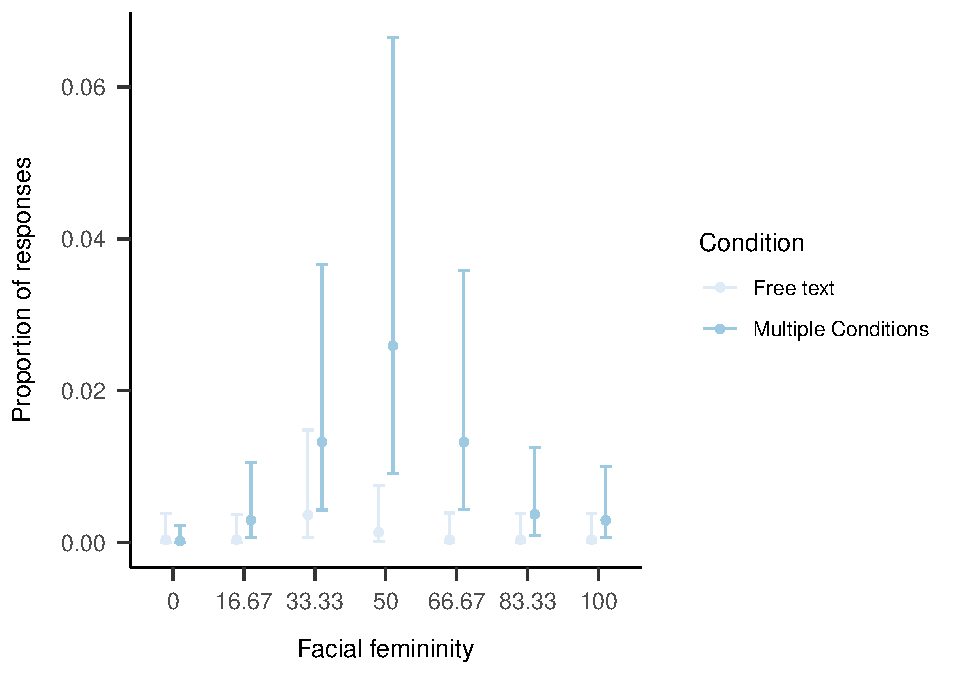
\includegraphics{resp_opts_manus23022_files/figure-latex/exp-one-inf-1.pdf}
\caption{\label{fig:exp-one-inf}Proportion of beyond-binary responses in the Mulitple categoreies and Free Text conditions}
\end{figure}

Model parameters are visualized in Figure~\ref{fig:exp-one-inf}. First, whether participants overall made more beyond-binary categorizations in the multiple categories condition than in the free text condition. The evidence suggests fairly convincingly that this is the case (OR = 0.02, CI ={[}0.00, 0.21{]}, BF\textsubscript{10}= 97.67). Additionally, based on the curve in Figure~\ref{fig:exp-one-inf}, we explored whether the evidence supported this difference at morph level 50. The evidence was in favor of this difference (OR = 0.02, CI ={[}0.00, 0.26{]}, BF\textsubscript{10}= 17). Lastly, we tested the difference using quadratic weights, though here the difference was inconclusive (OR = 0.82, CI = {[}0.44,1.58{]}, BF\textsubscript{10}= 0.53). \emph{I'm not sure how to interpret this last finding}.

Overall, though, the evidence suggests at least somewhat strongly that when participants have the option of using beyond-binary response options, they use them.

\hypertarget{rq2-which-categories-replace-the-non-binary-options}{%
\subsection{RQ2: Which categories replace the non-binary options?}\label{rq2-which-categories-replace-the-non-binary-options}}

\begin{table}

\caption{\label{tab:rq2-table}Relative predictive power of models describing the outcome on the categorization task}
\centering
\begin{threeparttable}
\begin{tabular}[t]{llccc}
\toprule
  & LOO difference & St. Error diff & LOO & St. Error LOO\\
\midrule
morph\_only & 0.00 & 0.00 & -1343.71 & 43.17\\
main\_effects & -1.85 & 0.86 & -1345.56 & 43.17\\
condition\_only & -4.98 & 5.26 & -1348.69 & 44.49\\
Null & -5.36 & 4.88 & -1349.07 & 44.12\\
interaction & -6.69 & 3.02 & -1350.40 & 43.48\\
\bottomrule
\end{tabular}
\begin{tablenotes}[para]
\item \textit{Note.} 
\item LOO diff refers to the difference in loo between the model and the most predictive model. The first row describes the most predictive model, which is why the difference is 0
\end{tablenotes}
\end{threeparttable}
\end{table}

To test this research question, we first carried out model comparison. The results of this are presented in Table~\ref{tab:rq2-table}. Although the Interaction model was the worst in terms of LOO-CV, the standard errors were quite large relative to the difference. For completeness we therefore carried out the contrast analyses using the Interaction model.

Based on the pattern in Figure~\ref{fig:descriptives}, the contrast that was chosen was at morph level 50. The evidence were slightly in favor of there being no difference between the multiple categories and the free text conditions (Estimate = 0.61, CI ={[}0.29, 1.28{]}, BF\textsubscript{01}= 4.79) and moderately in favor of no difference between multiple categories and binary categories conditions (Estimate = 0.76, CI ={[}0.37, 1.57{]}, BF\textsubscript{01}= 9.08)

\hypertarget{discussion}{%
\subsection{Discussion}\label{discussion}}

The results from experiment 1 suggest that some participants do use the beyond-binary options when they have them, however only when these are explicitly spelled out. When participants are implicitly able to enter whatever they like, most still fell back on using woman/man. Furthermore, the results suggests that overall, even when participants used the beyond-binary options, this did not systematically affect their overall pattern of responses in terms of woman and man categorizations.

\hypertarget{experiment-2}{%
\section{Experiment 2}\label{experiment-2}}

\hypertarget{overview}{%
\subsection{Overview}\label{overview}}

The purpose of experiment 2 was primarily to test the extent to which response options that do not frame women and men as two opposites reducerd categorical perception. To that end, we once again borrowed from the literature on self-categorization, this time using Bem's (1978) method of measuring gender on two separate scales.

If categorical perception occurs, we would expect that scores of femininity to be lower than the percentage of femininity in the faces. Furthermore, if response options change perceptions of gender as a category, we would expect there to be less categorical perception in the multiple categories option.

\hypertarget{method-1}{%
\subsection{Method}\label{method-1}}

\hypertarget{participants-1}{%
\subsubsection{Participants}\label{participants-1}}

Participants (\emph{N} = 49) were recruited through advertising online and on the university campus (\emph{M}\textsubscript{age}= 36.67, \emph{SD}\textsubscript{age} = 12.54). All participants were informed that participation was voluntary. In term of gender X women and Y men participated The participants were randomly allocated to conditions.

\hypertarget{stimuli-procedure}{%
\subsection{Stimuli \& Procedure}\label{stimuli-procedure}}

The stimuli and procedure for experiment 2 were identical to experiment 1. Experiment 2 differed only the response options conditions. For experiment 2, there response option conditions consisted of single dimension, which ranged from ``woman'' to ``man'' and ``multiple dimension'' which ranged from ``not woman'' to ``woman'' and ``not man'' to ``man''. For the multiple dimensions condition, participants rated the same faces according to both scales, but on separate trials. Although Bem (1978) used scales of femininity and masculinity, the present anchors were chosen based on evidence that people categorize those two scales differently depending on whether the categorize the faces as a woman or man.

\hypertarget{data-analysis-1}{%
\subsection{Data analysis}\label{data-analysis-1}}

\hypertarget{research-question-3-now-this-distinction-feels-like-it-makes-a-lot-less-sense}{%
\subsubsection{Research question 3 (Now this distinction feels like it makes a lot less sense\ldots)}\label{research-question-3-now-this-distinction-feels-like-it-makes-a-lot-less-sense}}

In research question three, we investigated whether participants displayed less categorical perception in the multiple dimensions condition compared to the single dimension condition. This could manifest as an interaction where mean ratings of faces are more extreme at both 33.37 morph level and 66.66 morph level. In other words, if categorial perception is reduced, we would expect to see an interaction depending on condition and morph level, but not a main effect. As research question 3 was less exploratory than 1 and 2, we simply fit an intearction model, a bayesian mixed-effects model with morph level and condition as fixed effects and participants and faces as varying intercepts (See supplemental material for full model specification). Using Savage-Dickey density ratios, we calculated the Bayes Factors for the contrasts between single dimension condition and multiple dimension at morph level 33.37 and 66.66 only.

\hypertarget{results-1}{%
\section{Results}\label{results-1}}

The mean ratings in both conditions are presented in Figure~\ref{fig:descriptives-two}.

\begin{figure}
\centering
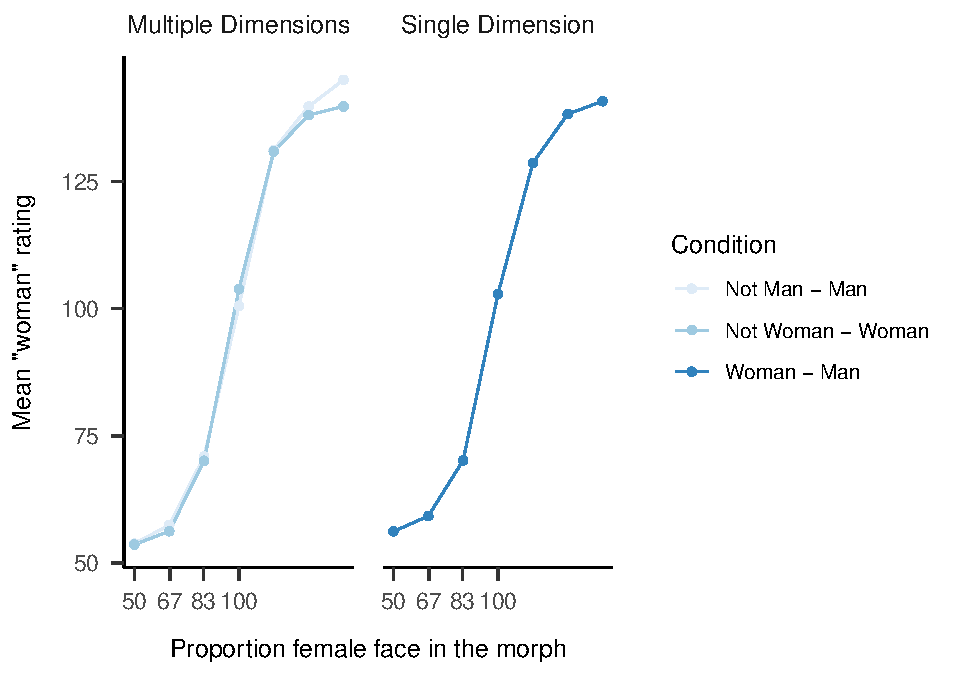
\includegraphics{resp_opts_manus23022_files/figure-latex/descriptives-two-1.pdf}
\caption{\label{fig:descriptives-two}Mean ratings of faces in Single dimension and multiple dimensions}
\end{figure}

\begin{figure}
\centering
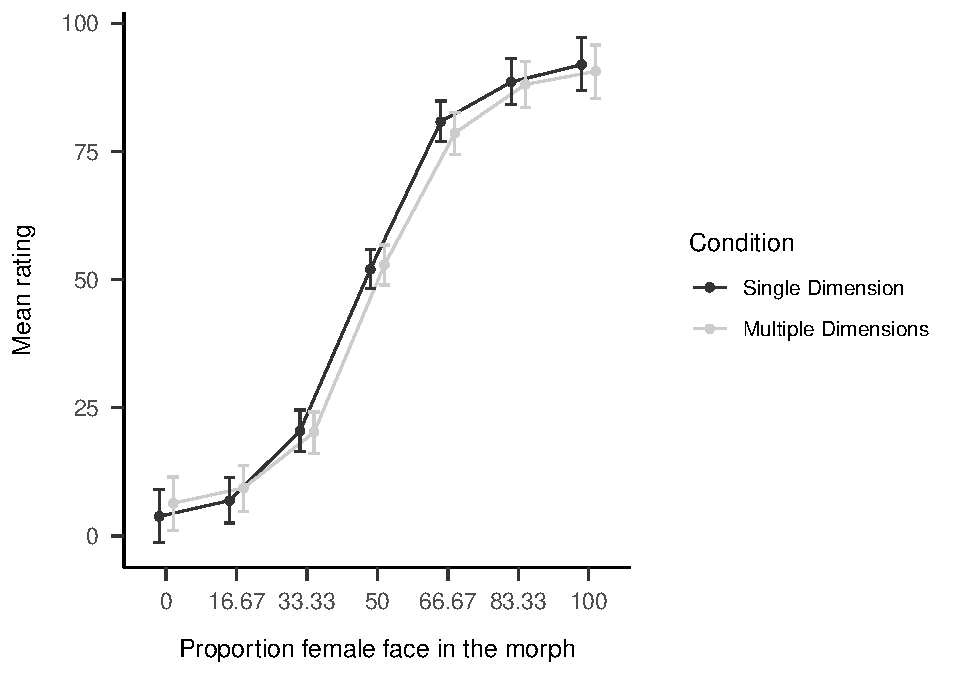
\includegraphics{resp_opts_manus23022_files/figure-latex/exp-two-inf-1.pdf}
\caption{\label{fig:exp-two-inf}Mean gender ratings in Single Dimension and Multiple Dimensions conditions}
\end{figure}

We compared the mean rating at 33.33 morph and at 66.67 morph for both conditions. At 33.33 the evidence strongly suggested that the two conditions were the same
(Estimate = 0.28, CI ={[}-3.91, 4.51{]}, BF\textsubscript{01}= 31.57). This was also the case at 66.67
(Estimate = 2.29, CI ={[}-2.03, 6.57{]}, BF\textsubscript{01}= 19.17). Overall, both conditions showed fairly strong tendencies toward categorical perception and they did not differ in this regard.

\hypertarget{discussion-1}{%
\section{Discussion}\label{discussion-1}}

Experiment 2 was designed to test whether response options which did not present women and men as opposing categories changed participants categorical perception. The results indicated that in terms of categorical perception, the two conditions were very similar, suggesting that the binary view of language is very strong and that participants do not change their view of gender depending on

\hypertarget{overall-discussion}{%
\section{Overall discussion}\label{overall-discussion}}

Overall, some important findings emerged from this experiment. First, there was strong evidence that participants will use beyond-binary actions to categorize faces, if given the options. It is also clear that providing these options do not change the overall distributions of scores.

Overall, this experiment yielded important findings regarding the use of non-binary response options in gender categorization. Specifically, the results provide strong evidence that participants will use beyond-binary options to categorize faces when such options are provided. Additionally, reponse options that pose men and women as not in opposition does not change participants ratings of their gender.

These findings are consistent with previous research, such as the work of Saperstein and Westbrook, which has highlighted the importance of including more options in measures of self-categorization. However, it is also important to note that the provision of non-binary options did not appear to significantly alter participants' perception of gender. This is a crucial point, as it indicates that including non-binary options in gender categorization measures can be done without compromising the study's ability to accurately assess participants' responses.

It is worth noting that this study only examined participants' stated categorizations, and it is possible that they may have made other categorizations internally that were not reflected in their responses. However, it is important to recognize that a purely behavioral study such as this cannot fully capture the neurological processes underlying gender perception, which may require more sophisticated techniques.

Based on these findings, we recommend that researchers carefully consider their goals when designing studies on gender categorization. For most studies, the inclusion of non-binary response options is a viable and ethical option that has the added benefit of avoiding micro-aggressions against transgender and non-binary participants. Ultimately, by taking a thoughtful and inclusive approach to gender categorization measures, researchers can improve the accuracy and validity of their results while respecting the diversity of human experiences.

\hypertarget{conclusion}{%
\paragraph{Conclusion}\label{conclusion}}

In conclusion, this experiment tested how the inclusion of response options which did not pose men and women as the only opposite gender affecte participants outcomes, in two studies.

\begin{verbatim}
Conclusion: End the discussion section with a brief summary of the study's main contributions and the overall conclusions that can be drawn from the results.
\end{verbatim}

\newpage

\hypertarget{references}{%
\section{References}\label{references}}

\hypertarget{refs}{}
\begin{CSLReferences}{1}{0}
\leavevmode\vadjust pre{\hypertarget{ref-R-papaja}{}}%
Aust, F., \& Barth, M. (2022). \emph{{papaja}: {Prepare} reproducible {APA} journal articles with {R Markdown}}. \url{https://github.com/crsh/papaja}

\leavevmode\vadjust pre{\hypertarget{ref-R-tinylabels}{}}%
Barth, M. (2022). \emph{{tinylabels}: Lightweight variable labels}. \url{https://cran.r-project.org/package=tinylabels}

\leavevmode\vadjust pre{\hypertarget{ref-R-brms_a}{}}%
Bürkner, P.-C. (2017). {brms}: An {R} package for {Bayesian} multilevel models using {Stan}. \emph{Journal of Statistical Software}, \emph{80}(1), 1--28. \url{https://doi.org/10.18637/jss.v080.i01}

\leavevmode\vadjust pre{\hypertarget{ref-R-brms_b}{}}%
Bürkner, P.-C. (2018). Advanced {Bayesian} multilevel modeling with the {R} package {brms}. \emph{The R Journal}, \emph{10}(1), 395--411. \url{https://doi.org/10.32614/RJ-2018-017}

\leavevmode\vadjust pre{\hypertarget{ref-R-brms_c}{}}%
Bürkner, P.-C. (2021). Bayesian item response modeling in {R} with {brms} and {Stan}. \emph{Journal of Statistical Software}, \emph{100}(5), 1--54. \url{https://doi.org/10.18637/jss.v100.i05}

\leavevmode\vadjust pre{\hypertarget{ref-R-gcookbook}{}}%
Chang, W. (2018). \emph{Gcookbook: Data for "r graphics cookbook"}. \url{https://CRAN.R-project.org/package=gcookbook}

\leavevmode\vadjust pre{\hypertarget{ref-R-Rcpp_b}{}}%
Eddelbuettel, D., \& Balamuta, J. J. (2018). {Extending extit{R} with extit{C++}: A Brief Introduction to extit{Rcpp}}. \emph{The American Statistician}, \emph{72}(1), 28--36. \url{https://doi.org/10.1080/00031305.2017.1375990}

\leavevmode\vadjust pre{\hypertarget{ref-R-Rcpp_a}{}}%
Eddelbuettel, D., \& François, R. (2011). {Rcpp}: Seamless {R} and {C++} integration. \emph{Journal of Statistical Software}, \emph{40}(8), 1--18. \url{https://doi.org/10.18637/jss.v040.i08}

\leavevmode\vadjust pre{\hypertarget{ref-R-bayesplot}{}}%
Gabry, J., Simpson, D., Vehtari, A., Betancourt, M., \& Gelman, A. (2019). Visualization in bayesian workflow. \emph{J. R. Stat. Soc. A}, \emph{182}, 389--402. \url{https://doi.org/10.1111/rssa.12378}

\leavevmode\vadjust pre{\hypertarget{ref-R-tidybayes}{}}%
Kay, M. (2022). \emph{{tidybayes}: Tidy data and geoms for {Bayesian} models}. \url{https://doi.org/10.5281/zenodo.1308151}

\leavevmode\vadjust pre{\hypertarget{ref-R-base}{}}%
R Core Team. (2022). \emph{R: A language and environment for statistical computing}. R Foundation for Statistical Computing. \url{https://www.R-project.org/}

\leavevmode\vadjust pre{\hypertarget{ref-R-ggplot2}{}}%
Wickham, H. (2016). \emph{ggplot2: Elegant graphics for data analysis}. Springer-Verlag New York. \url{https://ggplot2.tidyverse.org}

\leavevmode\vadjust pre{\hypertarget{ref-R-dplyr}{}}%
Wickham, H., François, R., Henry, L., \& Müller, K. (2022). \emph{Dplyr: A grammar of data manipulation}. \url{https://CRAN.R-project.org/package=dplyr}

\leavevmode\vadjust pre{\hypertarget{ref-R-tidyr}{}}%
Wickham, H., \& Girlich, M. (2022). \emph{Tidyr: Tidy messy data}. \url{https://CRAN.R-project.org/package=tidyr}

\end{CSLReferences}


\end{document}
